% Asset ID: AS1AlgebraicExpressionsTIKZ-006
% Source: Dr Frost rationalising denominator slides and transcript
% Related lesson section: Rationalising the Denominator, Worked Examples
% Purpose: Show why multiplying by the conjugate rationalises 1/(sqrt(2)+1).

\documentclass[tikz,border=8pt]{standalone}
\usetikzlibrary{arrows.meta,positioning,calc}

\begin{document}
\begin{tikzpicture}[
    font=\sffamily,
    arrow/.style={-{Latex[length=3mm]}, thick},
    box/.style={draw, rounded corners=4pt, thick, fill=gray!8, align=center, text width=4.4cm, minimum height=1.25cm},
    work/.style={draw, rounded corners=4pt, thick, fill=white, align=center, text width=5.4cm, minimum height=1.25cm},
    final/.style={draw, rounded corners=4pt, thick, fill=black, text=white, align=center, text width=5.4cm, minimum height=1.25cm}
]

\node[font=\sffamily\bfseries\Large] at (0,3.5)
{Rationalising with the conjugate};

\node[box] (start) at (-4.6,1.9)
{Start\\$\dfrac{1}{\sqrt2+1}$};

\node[box] (conj) at (0,1.9)
{Use conjugate\\$\sqrt2-1$};

\node[box] (multiply) at (4.6,1.9)
{Multiply by $1$\\$\dfrac{\sqrt2-1}{\sqrt2-1}$};

\draw[arrow] (start.east) -- (conj.west);
\draw[arrow] (conj.east) -- (multiply.west);

\node[work] (fraction) at (0,0.05)
{$\dfrac{1}{\sqrt2+1}\times\dfrac{\sqrt2-1}{\sqrt2-1}$\\[4pt]
$=\dfrac{\sqrt2-1}{(\sqrt2+1)(\sqrt2-1)}$};

\draw[arrow] (multiply.south west) -- (fraction.north east);

\node[work] (denom) at (-3.15,-2.0)
{$(\sqrt2+1)(\sqrt2-1)$\\[4pt]
$=(\sqrt2)^2-1^2$};

\node[work] (simplify) at (3.15,-2.0)
{$(\sqrt2)^2-1^2$\\[4pt]
$=2-1=1$};

\draw[arrow] (fraction.south west) -- (denom.north);
\draw[arrow] (denom.east) -- (simplify.west);

\node[final] (answer) at (0,-4.0)
{$\dfrac{1}{\sqrt2+1}=\sqrt2-1$};

\draw[arrow] (simplify.south west) -- (answer.north east);

\node[draw, rounded corners=4pt, thick, fill=gray!12, align=center, text width=10.6cm] at (0,-5.4)
{\textbf{Why it works:} $(a+b)(a-b)=a^2-b^2$, so the middle surd terms cancel.};

\end{tikzpicture}
\end{document}
